% -*- mode: LaTeX; TeX-PDF-mode: t; -*- # Tell emacs file type (for syntax coloring)
% Add the listed directories to the search path
% (allows easy moving of files around later)
% these paths are searched AFTER local config kpsewhich

% *.sty, *.cls
\makeatletter
\def\input@path{{@resources/texlive/texmf-local/tex/latex/}
        ,{@resources/texlive/texmf-local/bibtex/bst/},
        ,{@resources/texlive/texmf-local/bibtex/bib/},
        ,{@local/}
        }
\makeatother
\makeatletter
\def\bibinput@path{{@resources/texlive/texmf-local/tex/latex/}
        ,{@resources/texlive/texmf-local/bibtex/bst/},
        ,{@resources/texlive/texmf-local/bibtex/bib/},
        ,{@local/}
        }
\makeatother
  % allow latex to find custom stuff
% LaTeX path to the root directory of the current project, from the directory in which this file resides
% and path to econtexPaths which defines the rest of the paths like \FigDir
\providecommand{\econtexRoot}{}\renewcommand{\econtexRoot}{.}
 % Set paths (like, \LaTeXInputs) to find resources
\documentclass[\econtexRoot/Letter]{subfiles}
\onlyinsubfile{\externaldocument{\econtexRoot/Letter}} % Get xrefs -- esp to apndx -- from main file; only works if main file has already been compiled

\begin{document}
\notinsubfile{\renewcommand{\econtexRoot}{.}}

%\hypertarget{job-market-paper}{}
%\par\section{Job Market Paper}
%\notinsubfile{\label{sec:job-market-paper}}


Will has made substantial contributions to \href{https://github.com/econ-ark/HARK}{HARK}, an open-source Python toolkit for solving heterogeneous agent models that a team of collaborators and I have been developing for several years.  His contributions have been focused on developing methods to compute heterogeneous agent Jacobians. These Jacobians are essential for solving general equilibrium models with rich microeconomic heterogeneity following the Sequence Space Jacobian methodology by \cite{Auclert2021}.
% Please don't put in a cite key like \cite{Auclert2023} without including the corresponding bib entry.
Will has created several Jupyter notebooks illustrating how to use HARK to generate these Jacobians and solve general equilibrium HA models. % CDC to DuW: Alan has figured out how to make a direct link to a page that shows stats about his contributions to HARK; please get the parallel link for your contributions and edit this doc to include that link

He developed a notebook for simulating large heterogeneous agent economies with HARK (\href{https://github.com/econ-ark/HARK/blob/master/examples/ConsNewKeynesianModel/Transition_Matrix_Example.ipynb}{Simulation notebook}) and another for computing heterogeneous agent Jacobians (\href{https://github.com/econ-ark/HARK/blob/master/examples/ConsNewKeynesianModel/Jacobian_Example.ipynb}{Jacobian notebook}). He has also integrated his methods with the \href{https://github.com/shade-econ/sequence-jacobian}{Sequence Space Jacobian toolkit} to solve HANK models (\href{https://github.com/econ-ark/HARK/blob/master/examples/ConsNewKeynesianModel/SSJ_example.ipynb}{HANK notebook}) and a Krusell-Smith model without aggregate uncertainty (\href{https://github.com/econ-ark/HARK/blob/master/examples/ConsNewKeynesianModel/KS-HARK-presentation.ipynb}{Krusell-Smith Notebook}).

For the past two years I have invited Will to lecture on Sequence Space Jacobian methods in my Ph.D.\ computational economics course, for which he created a notebook explaining the mathematics and intuition behind the method (\href{https://github.com/econ-ark/HARK/blob/master/examples/ConsNewKeynesianModel/SSJ_explanation.ipynb}{notebook here}). During his tenure as a Ph.D. intern at the Bank of England, Will employed his computational skills on solving general equilibrium models with rich microeconomic features to solve a HANK model with housing as a discrete choice (\href{https://github.com/wdu9/HANK_Housing_Block}{Slides and Code}). Heterogeneous agent models with discrete choice introduce a discrete continuous interaction that makes these models challenging to solve. An overview of the computational tools Will has developed can be found \href{https://www.william-du.com/computational-tools}{here}.


%Will has also made important contributions to HARK, an open source python toolkit for solving heterogeneous agent models. His contributions have largely focused on developing methods that compute heterogeneous agent Jacobians. These Jacobians are an essential object in solving general equilibrium models with rich microeconomic heterogeneity following the Sequence Space Jacobian methodology of \cite{Auclert2023}.  Will has produced several Jupyter notebooks demonstrating how to use the HARK code to produce these Jacobians and then solve general equilibrium models with rich micro heterogeneity. In particular, he has written notebooks on how to utilize his methods to simulate large heterogeneous agent economies with HARK (\href{https://github.com/econ-ark/HARK/blob/master/examples/ConsNewKeynesianModel/Transition_Matrix_Example.ipynb}{Simulation notebook}) and how to compute heterogeneous agent Jacobians (\href{https://github.com/econ-ark/HARK/blob/master/examples/ConsNewKeynesianModel/Jacobian_Example.ipynb}{Jacobian notebook}). In turn, Will has used the methods he constructed in these notebooks to write additional notebooks on how to combine HARK and the \href{https://github.com/shade-econ/sequence-jacobian}{Sequence Space Jacobian toolkit} to solve HANK models (\href{https://github.com/econ-ark/HARK/blob/master/examples/ConsNewKeynesianModel/SSJ_example.ipynb}{HANK notebook}) and a Krusell Smith model without aggregate uncertainty (\href{https://github.com/econ-ark/HARK/blob/master/examples/ConsNewKeynesianModel/KS-HARK-presentation.ipynb}{Krusell Smith Notebook}). For two consecutive years, I have invited Will to give a lecture on Sequence Space Jacobian methods in my Ph.D. computational economics course. For his lecture, Will created a jupyter notebook detailing the mathematics and intuition of the method (\href{https://github.com/econ-ark/HARK/blob/master/examples/ConsNewKeynesianModel/SSJ_explanation.ipynb}{notebook here}). 









%in a particular dimension: The consequences of a recession for subsequent output. To gauge the magnitude of the effects, Will does an exercise to evaluate the aftermath of the Great Recession in the United States and in the Euro zone, motivated by the fact that in Europe the byword for the fiscal response to the GR was ``austerity'' while in the US there was considerable stimulus (and a litany of criticism that the US should be pursuing austerity not stimulus). In Will's model, as in the data, the stimulative policy results in a much lower permanent drop in GDP than the austerity policy, corresponding to the actual outcomes in the US versus Europe.

%Consistent with the old literature suggesting that there is a unit root in GDP, Will finds that in his HANK model a recession results in a permanent reduction in the level of GDP because the shocks to human capital are permanent. These results connect not only with the old unit root and ``hysteresis'' literatures, but also with the newer ``secular stagnation'' literature. 





% Put here a link to the abstract of the JMP:

%%% Template for any figures
%\begin{figure}[ht!]
%	\centering
%	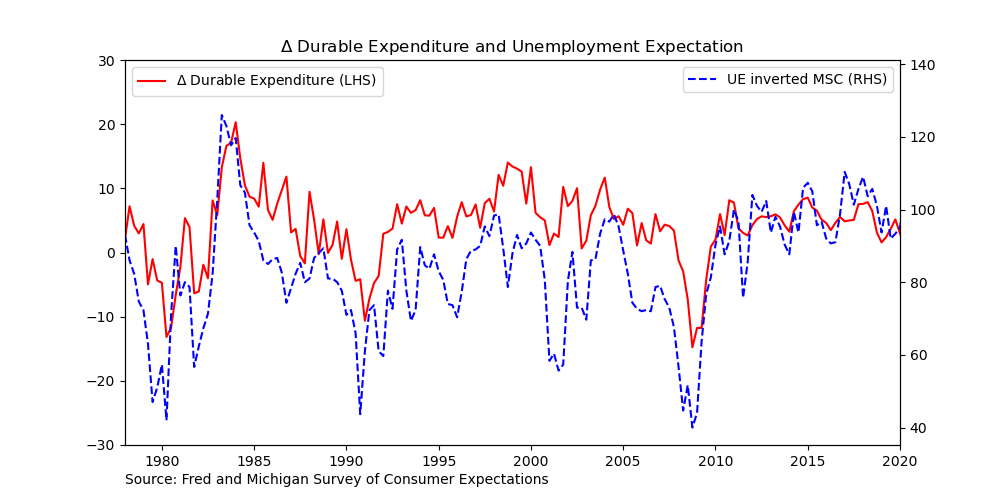
\includegraphics[width = 0.8\textwidth]{\FigDir/dur_vs_exp_emp.png}
	%\caption{Durable Expenditure and Expected Unemployment Rate} \label{fig:dur_vs_exp_emp}
%\end{figure}

\onlyinsubfile{% Allows two (optional) supplements to hard-wired \texname.bib bibfile:
% system.bib is a default bibfile that supplies anything missing elsewhere
% Add-Refs.bib is an override bibfile that supplants anything in \texfile.bib or system.bib
\provideboolean{AddRefsExists}
\provideboolean{systemExists}
\provideboolean{BothExist}
\provideboolean{NeitherExists}
\setboolean{BothExist}{true}
\setboolean{NeitherExists}{true}

\IfFileExists{\econtexRoot/Add-Refs.bib}{
  % then
  \typeout{References in Add-Refs.bib will take precedence over those elsewhere}
  \setboolean{AddRefsExists}{true}
  \setboolean{NeitherExists}{false} % Default is true
}{
  % else
  \setboolean{AddRefsExists}{false} % No added refs exist so defaults will be used
  \setboolean{BothExist}{false}     % Default is that Add-Refs and system.bib both exist
}

% Deal with case where system.bib is found by kpsewhich
\IfFileExists{/usr/local/texlive/texmf-local/bibtex/bib/system.bib}{
  % then
  \typeout{References in system.bib will be used for items not found elsewhere}
  \setboolean{systemExists}{true}
  \setboolean{NeitherExists}{false}
}{
  % else
  \typeout{Found no system database file}
  \setboolean{systemExists}{false}
  \setboolean{BothExist}{false}
}

\ifthenelse{\boolean{showPageHead}}{ %then
  \clearpairofpagestyles % No header for references pages
  }{} % No head has been set to clear

\ifthenelse{\boolean{BothExist}}{
  % then use both
  \typeout{bibliography{\econtexRoot/Add-Refs,\econtexRoot/\texname,system}}
  \bibliography{\econtexRoot/Add-Refs,\econtexRoot/\texname,system}
  % else both do not exist
}{ % maybe neither does?
  \ifthenelse{\boolean{NeitherExists}}{
    \typeout{bibliography{\texname}}
    \bibliography{\texname}}{
    % no -- at least one exists
    \ifthenelse{\boolean{AddRefsExists}}{
      \typeout{bibliography{\econtexRoot/Add-Refs,\econtexRoot/\texname}}
      \bibliography{\econtexRoot/Add-Refs,\econtexRoot/\texname}}{
      \typeout{bibliography{\econtexRoot/\texname,system}}
      \bibliography{        \econtexRoot/\texname,system}}
  } % end of picking the one that exists
} % end of testing whether neither exists
}

\ifthenelse{\boolean{Web}}{}{
  \onlyinsubfile{\captionsetup[figure]{list=no}}
  \onlyinsubfile{\captionsetup[table]{list=no}}
  \end{document}	\endinput
}

